\section{Historical Evolution}
\label{sec:history}

\begin{figure*}[t]
  \centering
  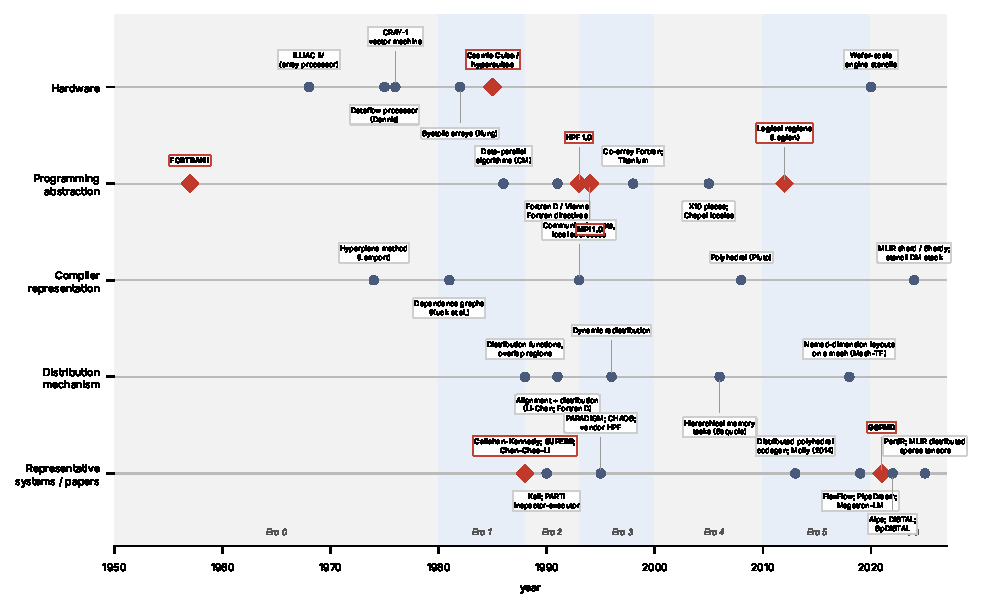
\includegraphics[width=\textwidth]{timeline.pdf}
  \caption{Timeline 1950--2026 with lanes for hardware, programming abstraction, compiler representation, distribution mechanism, and representative systems. Diamonds mark transitions that open a new era. Each event is tied to a catalog entry; era boundaries are provisional.}
  \label{fig:timeline}
\end{figure*}

Fig.~\ref{fig:timeline} and Table~\ref{tab:eras} organise the catalog into seven provisional eras. Each subsection ends with what changed, what remained, and the limitation that motivated the next era.

\subsection{Era 1: emergence (c.~1980--1987)}
\fact{Message-passing multicomputers made private memories and explicit communication the programmer's responsibility; the Cosmic Cube is the reference machine of this class~\cite{seitz1985cosmic}.} \todo{Add the early source-to-source and placement systems of this period once their records exist.}
\emph{Synthesis.} \infer{What changed: programmers faced private memories. What remained: sequential loop analysis. Limitation: all communication was hand-written, which motivated the compiler efforts of the next era.}

\subsection{Era 2: global arrays and data decomposition (c.~1988--1992)}
\fact{Zima, Bast and Gerndt's SUPERB system is described as a tool for semi-automatic MIMD/SIMD parallelisation~\cite{zima1988superb}.} \todo{Read \cite{gerndt1990updating} and state what it contributes to the handling of non-local copies in local computation.} \fact{Kali compiled global-name-space parallel loops over explicitly distributed arrays~\cite{mehrotra1990kali,koelbel1991compiling}.} \fact{Vienna Fortran extended Fortran with distribution, alignment and dynamic-distribution declarations~\cite{chapman1991vienna,chapman1992vienna}.} \fact{Fortran~D introduced decompositions and alignment with optimisations such as message vectorisation, and the 1992 evaluation measured the effect of each optimisation on an iPSC/860~\cite{hiranandani1991fortrand,hiranandani1992evaluation}.} \fact{Gupta and Banerjee chose one distribution per array by combining constraints weighted by estimated execution-time penalties~\cite{gupta1992automatic}.} \fact{Koelbel derived closed forms for communication and iteration sets of forall loops over block and cyclic arrays~\cite{koelbel1991regular}.} \fact{The PARTI runtime generated schedules for irregular loops whose access patterns are known only at run time~\cite{saltz1990runtime,saltz1991multiprocessor}.}
\emph{Synthesis.} \infer{What changed: data ownership became a compiler-visible object, and communication moved from the programmer into the compiler. What remained: dependence analysis from the foundations. Limitation: the systems handled regular affine code, and the choice of distribution was left to a costly or manual process, which motivated the standard language of the next era.}

\subsection{Era 3: HPF, MPI, and compiler maturity (c.~1993--2000)}
\fact{HPF 1.0 standardised ALIGN, DISTRIBUTE, TEMPLATE and PROCESSORS, with FORALL and INDEPENDENT~\cite{hpfforum1993spec,loveman1993hpf}.} \fact{Benkner and Zima's 1999 overview describes the compilation techniques of the decade: distribution and alignment processing, local index sets, owner-computes translation of array statements, and an inspector/executor scheme for irregular code~\cite{benkner1999compiling}.} \fact{Research compilers in this period include Fortran~90D/HPF~\cite{bozkus1993fortran90d}, PARADIGM~\cite{banerjee1995paradigm,su1995advanced} and Rogers and Pingali's Id-based compiler~\cite{rogers1994compiling}; Digital's HPF 1.1 compiler was a production product~\cite{harris1995dechpf}, and IBM's pHPF was a prototype for SP machines~\cite{gupta1995hpf}.} \fact{Closed-form communication sets for block-cyclic distributions were given by Chatterjee et al.~\cite{chatterjee1993generating}, and the redistribution problem was analysed by Ramaswamy et al.~\cite{ramaswamy1996redistribution} and Palermo et al.~\cite{palermo1996dynamic}.} \fact{MPI was standardised as the explicit alternative~\cite{mpiforum1994standard}, with MPICH as a portable implementation~\cite{gropp1996mpich}.} \fact{Kennedy, Koelbel and Zima's retrospective gives the causal account of why HPF lost most of its user base~\cite{kennedy2007rise}, and Loveman's article lists irregular and user-defined distributions among HPF's missing capabilities~\cite{loveman1993hpf}.}
\emph{Synthesis.} \infer{What changed: a standard distribution language and mature closed-form communication generation. What remained: owner-computes and block and cyclic distributions. Limitation: irregular codes were poorly served, and compiler performance was unpredictable, so practitioners used MPI directly.}

\subsection{Era 4: MPI dominance and alternative models (c.~2000--2010)}
\fact{Co-Array Fortran extends Fortran~95 with co-dimensions that name remote data by image index~\cite{numrich1998coarray}; Titanium is a Java dialect with a partitioned global address space and domain-based arrays~\cite{yelick2007titanium}; and the Berkeley UPC compiler translates UPC to C over GASNet~\cite{chen2003upc}.} \fact{Chapel presents user-definable distributions over locales as a global-view alternative to fixed directive sets~\cite{chamberlain2007chapel}.} \fact{Sequoia programs are hierarchies of tasks whose arguments describe data movement through a model of machine memory~\cite{fatahalian2006sequoia}, and Baskaran et al.\ allocate scratchpad buffers and generate movement code for explicitly managed memories~\cite{baskaran2008automatic}.} \fact{Tang and Xue generate SPMD code for rectangularly tiled, skewed iteration spaces with the computer-owns rule~\cite{tang2000tiled}.} \fact{The Pluto polyhedral optimiser~\cite{bondhugula2008pluto} provides the transformations that later distributed-memory generators build on.}
\emph{Synthesis.} \infer{What changed: distribution moved from directives into language types, domain maps and memory hierarchies. What remained: the owner concept. Limitation: adoption stayed limited, and automatic distribution was rarely used in production. \todo{Add the Berkeley UPC and HPCS evaluations, and verify the adoption claim against \cite{kennedy2007rise}.}}

\subsection{Era 5: compiler/runtime co-design and accelerators (c.~2010--2019)}
\fact{Bondhugula generated MPI communication for affine loop nests from polyhedral dependences, with flow-out and write-out sets and run-time helper functions for partners~\cite{bondhugula2011automatic,bondhugula2013compiling}; Molly does the same inside LLVM and Polly with element-level home locations~\cite{kruse2014molly}; and Dathathri et al.\ target a dataflow runtime~\cite{dathathri2014thesis,dathathri2016compiling}.} \fact{Legion expresses locality and independence with logical regions and a mapper interface~\cite{bauer2012legion}, and Regent compiles a sequential-looking language with privilege checking onto Legion~\cite{slaughter2015regent}.} \fact{Mesh-TensorFlow introduced named-dimension layouts on a processor mesh~\cite{shazeer2018meshtf}; FlexFlow searched per-operator parallelisation configurations with a simulator~\cite{jia2019flexflow}; GPipe and PipeDream established pipeline parallelism for training~\cite{huang2019gpipe,narayanan2019pipedream}; and Megatron-LM implemented tensor parallelism by hand~\cite{shoeybi2019megatron}.}
\emph{Synthesis.} \infer{What changed: accelerators and ML workloads became the driver, and representations diversified into polyhedral, region-based and mesh forms. Limitation: each system covered one domain, and the plan for an ML model was still largely a manual choice.}

\subsection{Era 6: mesh sharding, ML systems, spatial accelerators (c.~2020--2026)}
\todo{Read \cite{lepikhin2020gshard} and state its contribution from the text; it is catalogued as the predecessor of GSPMD.} \fact{GSPMD generalised annotation completion and per-operator SPMD partitioning~\cite{xu2021gspmd}. Alpa combines inter- and intra-operator parallelism~\cite{zheng2022alpa}, and PartIR composes partitioning strategies as tactics~\cite{alabed2025partir}.}
\emph{Synthesis.} \infer{What changed: the programmer writes an unpartitioned model and a mesh, and the compiler propagates the layout. Limitation: dynamic, irregular and memory-capacity-limited workloads remain weakly handled; Section~\ref{sec:open} returns to this.}
